\section{Proposed Visualization}

\subsection{Data preparation}

The raw SIH/SUS extract is too large to query while the user waits.
It holds about 183 million admissions in a 26\,GB table, and a single aggregation over one year already takes tens of seconds.
To keep the interface responsive, we move all of the heavy work to an offline step that runs once.

This step makes one pass over the fact table.
It joins each admission to the municipality where the patient lives and to the municipality of the hospital, then groups the rows by origin, destination, specialty, year, and month.
The result is a small set of tables, the largest with 13.5 million rows, that the application reads in place of the raw data.
Figure~\ref{fig:architecture} shows this pipeline.
Queries against these tables return in under 100 milliseconds, so filtering and navigation feel immediate.

\begin{figure}[t]
  \centering
  \begin{tikzpicture}[
    node distance=5mm,
    box/.style={draw, rounded corners, align=center, inner sep=4pt,
                font=\small, text width=0.80\columnwidth},
    arr/.style={-{Latex[length=2mm]}, thick}
  ]
    \node[box] (raw)  {Raw SIH/SUS in DuckDB\\26\,GB, 183M admissions};
    \node[box, below=of raw]  (etl)  {Offline ETL, run once\\join residence and hospital municipalities, group by origin, destination, specialty, year, month};
    \node[box, below=of etl]  (agg)  {Aggregate tables\\\texttt{fato\_fluxo} (13.5M rows) and per-municipality tables};
    \node[box, below=of agg]  (api)  {FastAPI service\\serves JSON in under 100\,ms};
    \node[box, below=of api]  (front){React and deck.gl\\interactive flow map};
    \draw[arr] (raw)  -- (etl);
    \draw[arr] (etl)  -- (agg);
    \draw[arr] (agg)  -- (api);
    \draw[arr] (api)  -- (front);
  \end{tikzpicture}
  \caption{%
    Data pipeline.
    All aggregation runs once, offline, turning the 183 million row table into small tables that the service can query in under 100 milliseconds.%
  }
  \label{fig:architecture}
\end{figure}

\subsection{The flow map}

We draw each hospitalization flow as a curved arc from the patient's residence to the hospital municipality.
The width of the arc grows with the number of admissions, so the thickest arcs mark the busiest routes.
Color marks the direction relative to the place in focus, with arcs that leave a region drawn in orange and arcs that arrive drawn in blue.

A choropleth sits behind the arcs and fills each state or city with one chosen metric.
The default metric is the attraction balance, the number of admissions a place receives minus the number its own residents generate.
Blue means the place treats more patients than it sends away, and red means the opposite.
City nodes appear as circles sized by the number of admissions that pass through them.
A dark basemap keeps the arcs and nodes easy to read.

\subsection{Three levels of detail}

The map follows the principle of overview first, then zoom and filter, then details on demand~\cite{Shneiderman1996EyesHaveIt}.
It opens at the national level, where the 27 states are the nodes and the arcs show flows between states.
Clicking a state opens the state level, where its municipalities become the nodes and the arcs show flows inside the state and toward other states.
Clicking a city opens the city level, which shows every flow that touches that city across the country.
Figure~\ref{fig:drilldown} shows the three levels for Rio Grande do Sul.
A breadcrumb at the top records the path and lets the user step back, and the camera flies to each new selection.

\begin{figure}[t]
  \centering
  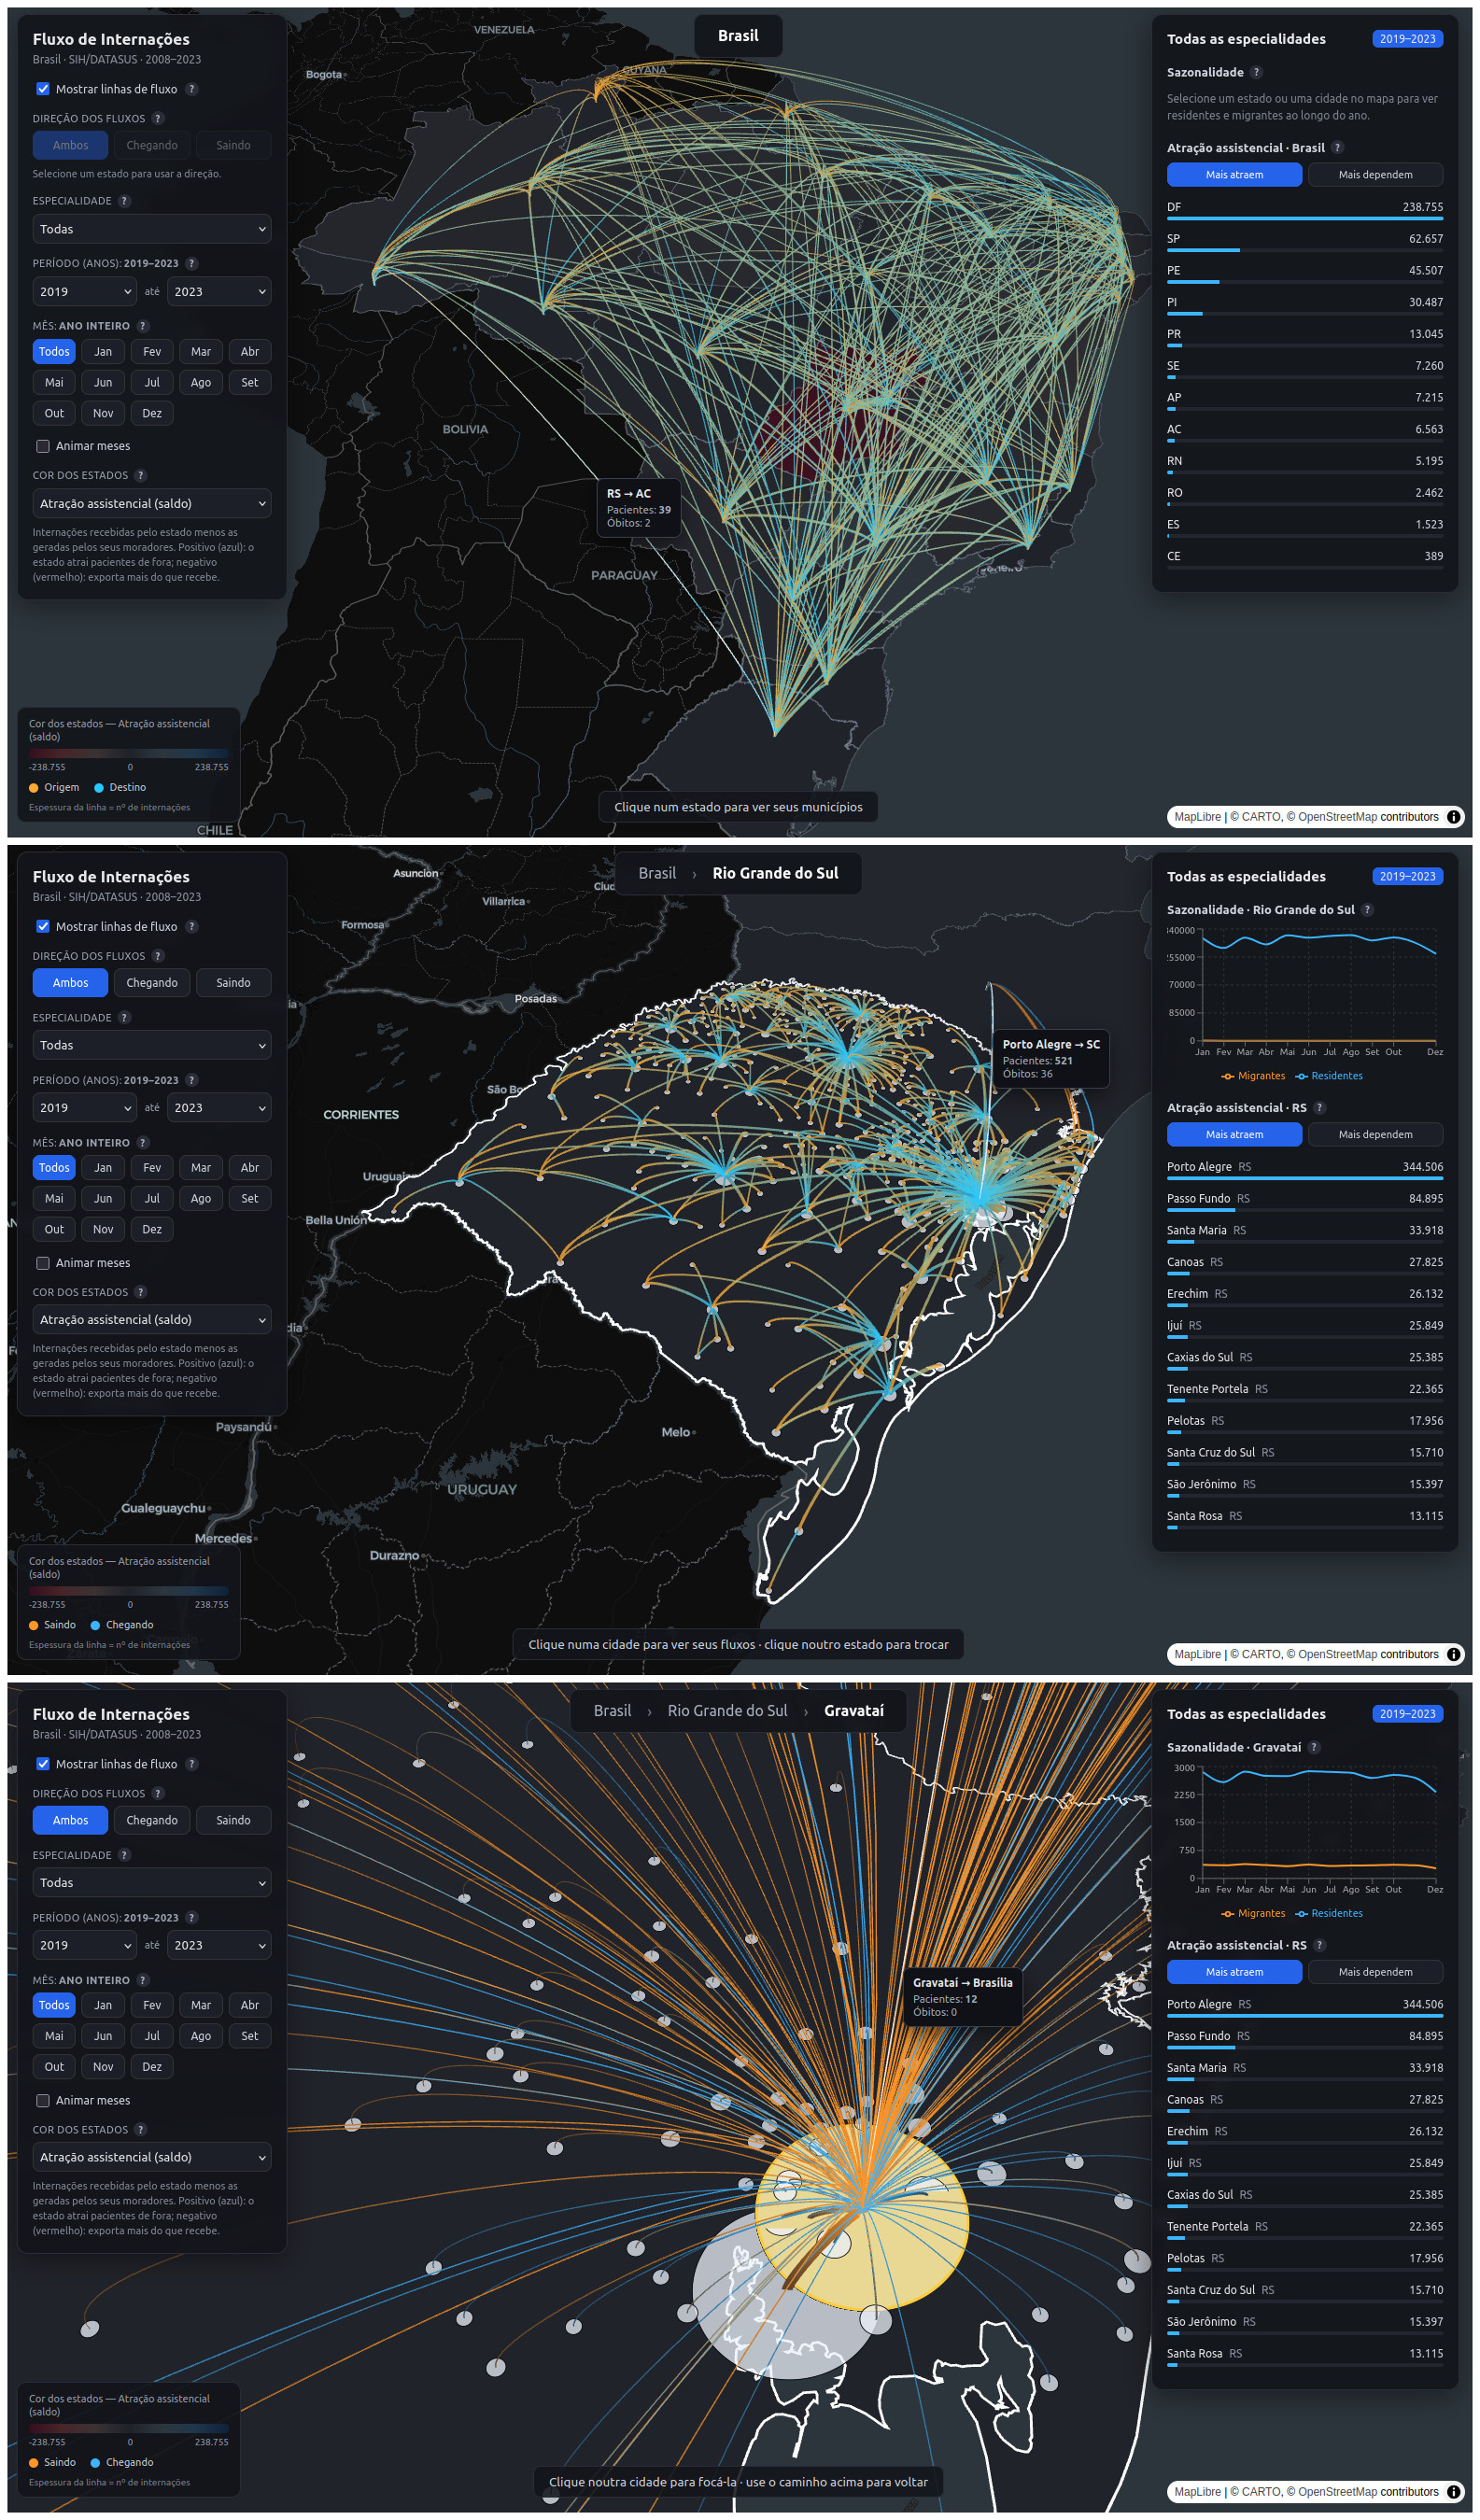
\includegraphics[width=0.78\columnwidth]{national-to-city-view.jpeg}
  \caption{%
    The three levels of the flow map for Rio Grande do Sul.
    Top: the national level, with states as nodes and arcs between them.
    Middle: the state level, with municipalities as nodes.
    Bottom: the city level, showing every flow that touches the selected city.%
  }
  \label{fig:drilldown}
\end{figure}

\subsection{Filters and animation}

Filters narrow the data without leaving the map.
The user can pick a medical specialty, a range of years, and a single month, and can change the metric used for the choropleth.
A direction control limits the arcs to those leaving or arriving at the focus, which removes clutter when a city has many connections.
A further option plays the twelve months in sequence, so seasonal change appears as motion on the map.

\subsection{Analytical panels}

Two side panels turn the map into direct answers.
The ranking panel lists the places with the strongest attraction balance, and a toggle switches between the cities that attract the most patients and the cities that most depend on others.
Figure~\ref{fig:ranking} shows this ranking for Rio Grande do Sul, with Porto Alegre as the clear hub and Viam\~{a}o among the most dependent municipalities.

The second panel plots a monthly time series that separates resident admissions from incoming ones.
This shows whether a seasonal peak comes from local patients or from people arriving from elsewhere.

The arc colors make the same contrast visible on the map.
Figure~\ref{fig:contrast} compares the two municipalities from the ranking, filtered to facial surgery between 2015 and 2023.
Porto Alegre is covered by blue arcs that arrive from across the state and from other states, while Viam\~{a}o shows mostly orange arcs that leave for nearby cities.

\begin{figure}[t]
  \centering
  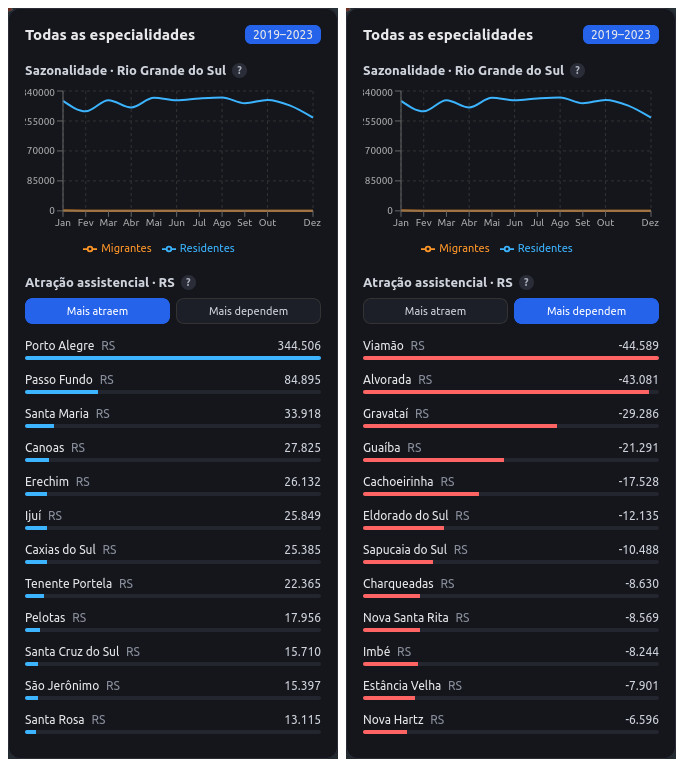
\includegraphics[width=0.92\columnwidth]{attract-vs-depend-more.jpeg}
  \caption{%
    The attraction ranking for Rio Grande do Sul, all specialties, 2019 to 2023.
    Left: the municipalities that attract the most patients, led by Porto Alegre.
    Right: the municipalities that most depend on care elsewhere, led by Viam\~{a}o.
    Bar length encodes the attraction balance, blue for positive and red for negative.%
  }
  \label{fig:ranking}
\end{figure}

\begin{figure}[t]
  \centering
  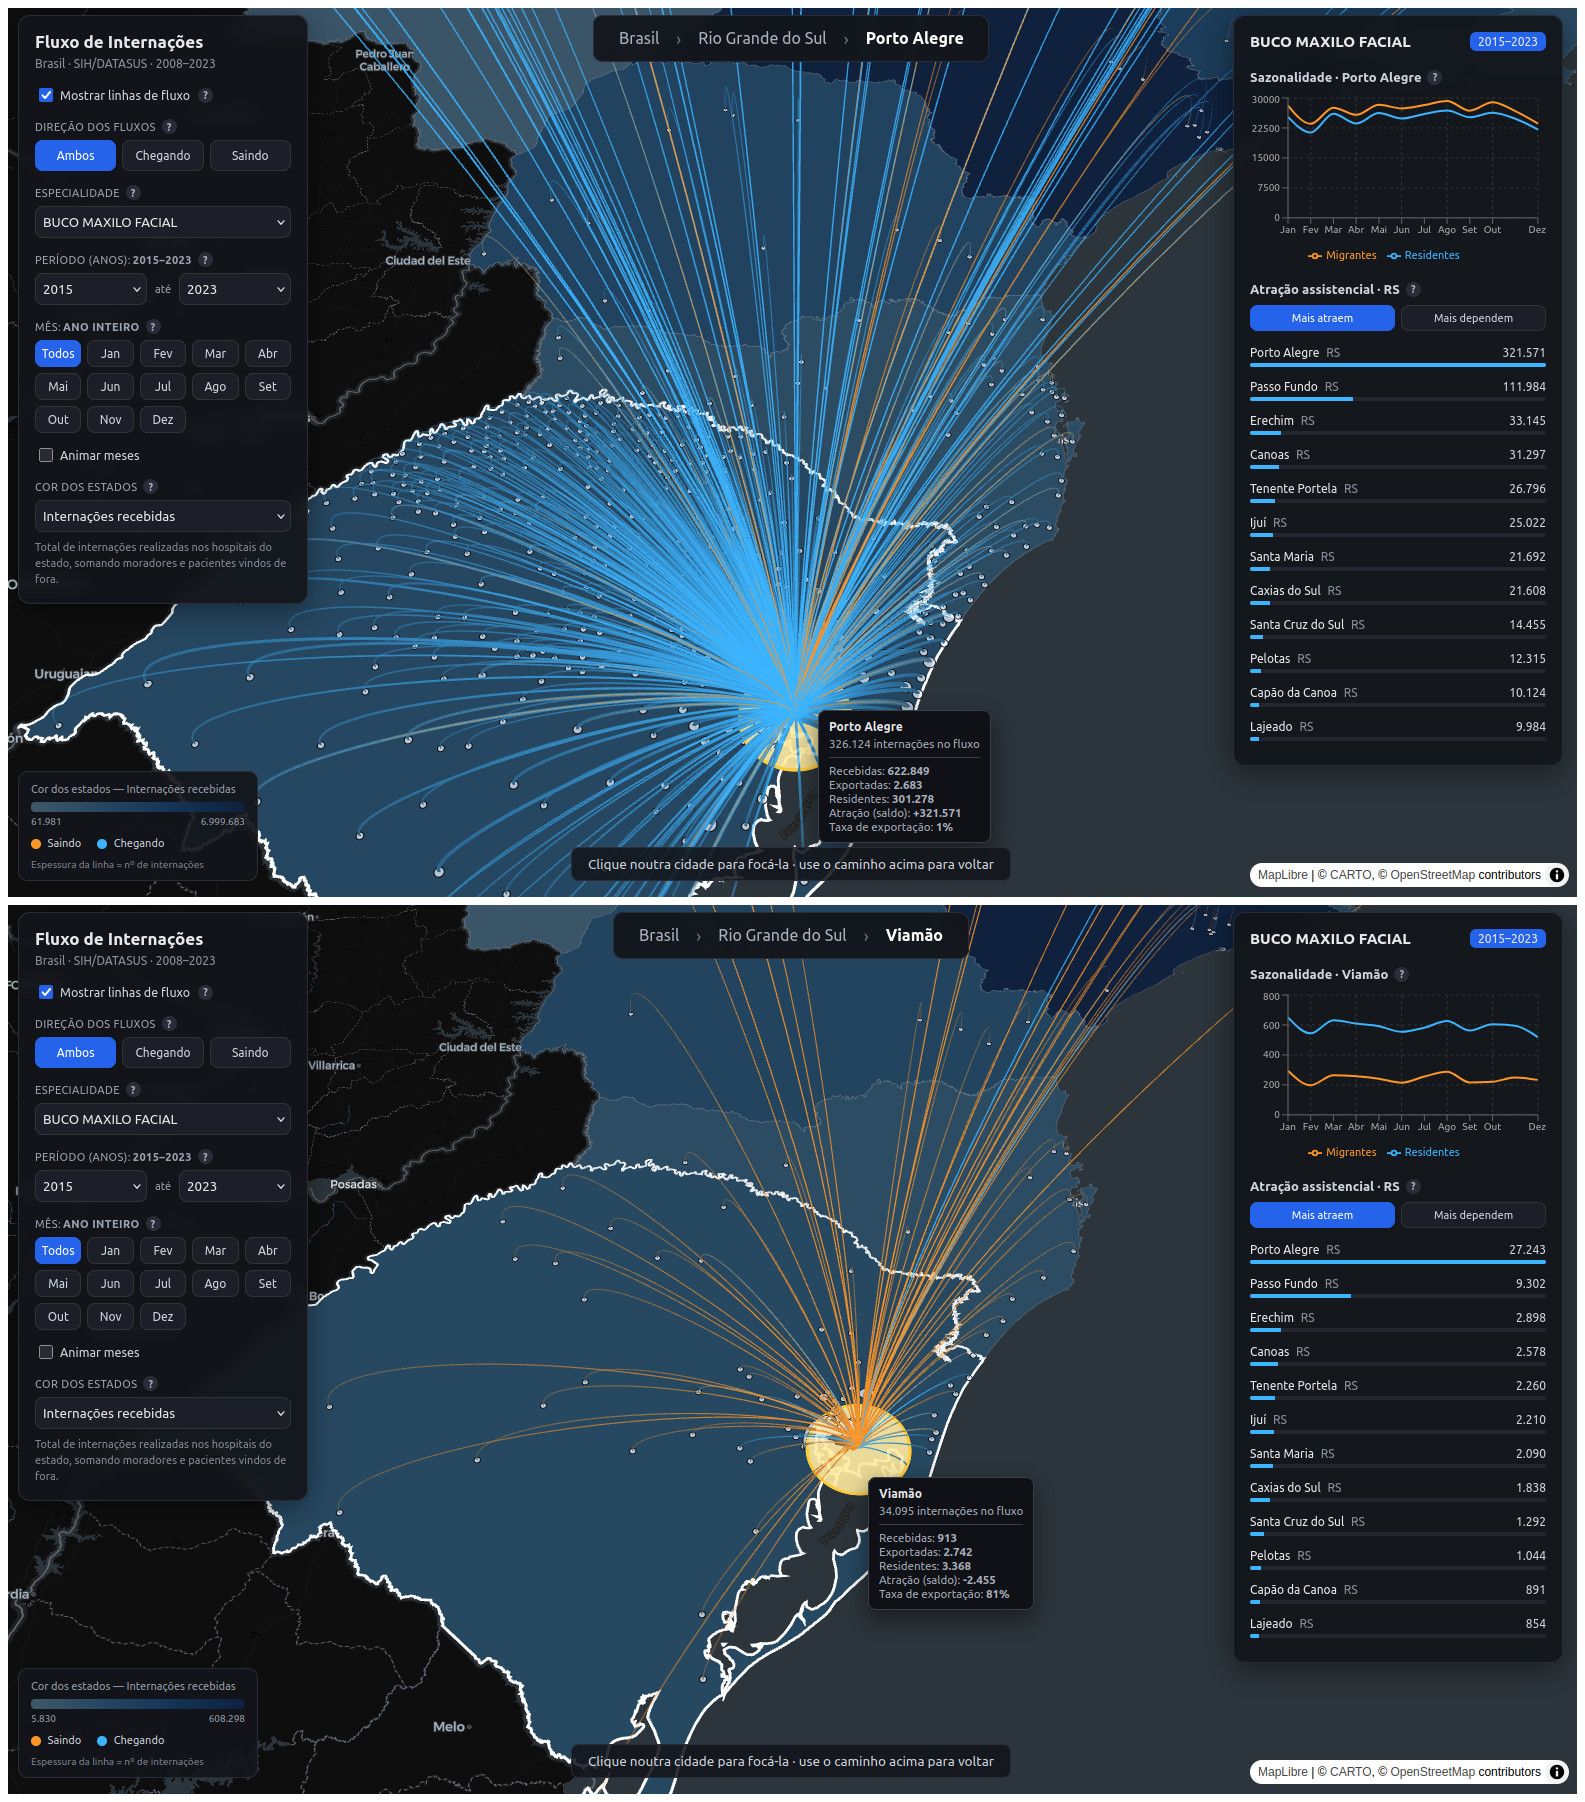
\includegraphics[width=0.92\columnwidth]{poa-vs-viamao-buco-maxilo-facial.jpeg}
  \caption{%
    City level view of two municipalities in Rio Grande do Sul for facial surgery (Buco Maxilo Facial), 2015 to 2023.
    Porto Alegre (top) is reached by many blue arcs, since patients arrive from across the state and from other states.
    Viam\~{a}o (bottom) shows mostly orange arcs, since its residents leave for other cities.
    The two were the top attracting and top dependent municipalities in the ranking of Figure~\ref{fig:ranking}.%
  }
  \label{fig:contrast}
\end{figure}
